
\begin{figure}[ht]
\centering
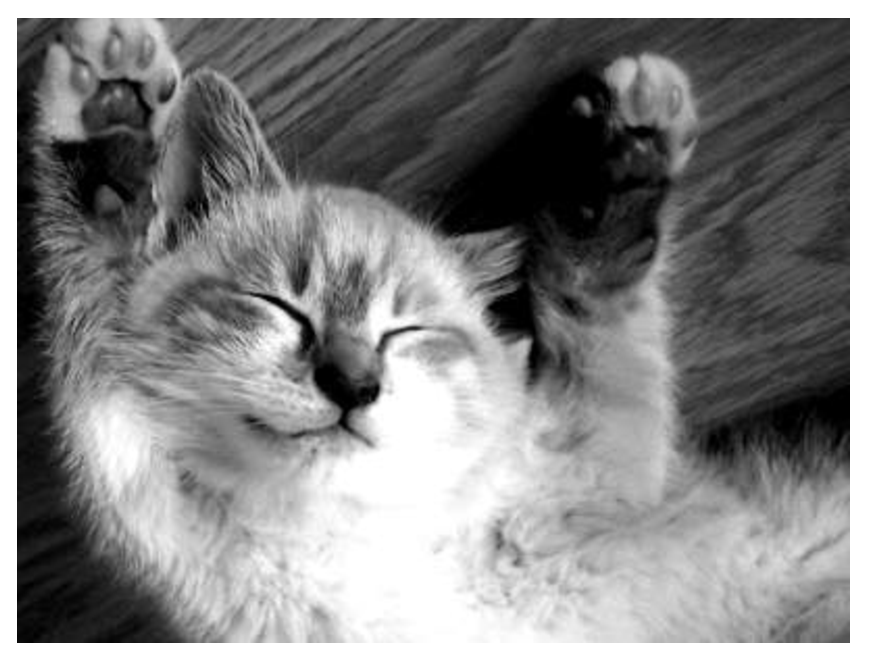
\includegraphics[width=0.8\textwidth]{./chapters/demonstration/no_release/kitten.eps}
\caption[$^{235}U$ residence. Lumped Parameter  <+Component+> No Release.]{
For <+CASE+> case in which total containment in the <+component+> is assumed 
($F_{d,<+comp+>}=0$), $^{235}U$ travels through <++> components ($F_d = 0.1$) before 
permanent residence in the <+component+> component.
}
\label{fig:lpIall}
\begin{minipage}[b]{0.45\linewidth}

  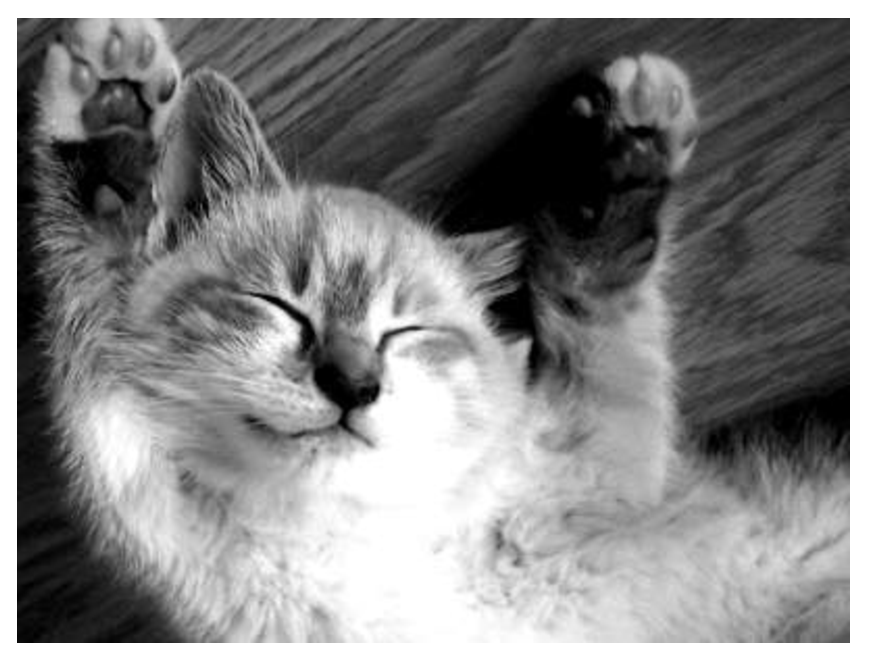
\includegraphics[width=\textwidth]{./chapters/demonstration/no_release/kitten.eps}
  \caption[1DI Waste Form Contaminants.]{
    Waste Form 5 ($F_d = 0.1$) releases material with degradation. 
    }
  \label{fig:lpIwf5}
  
  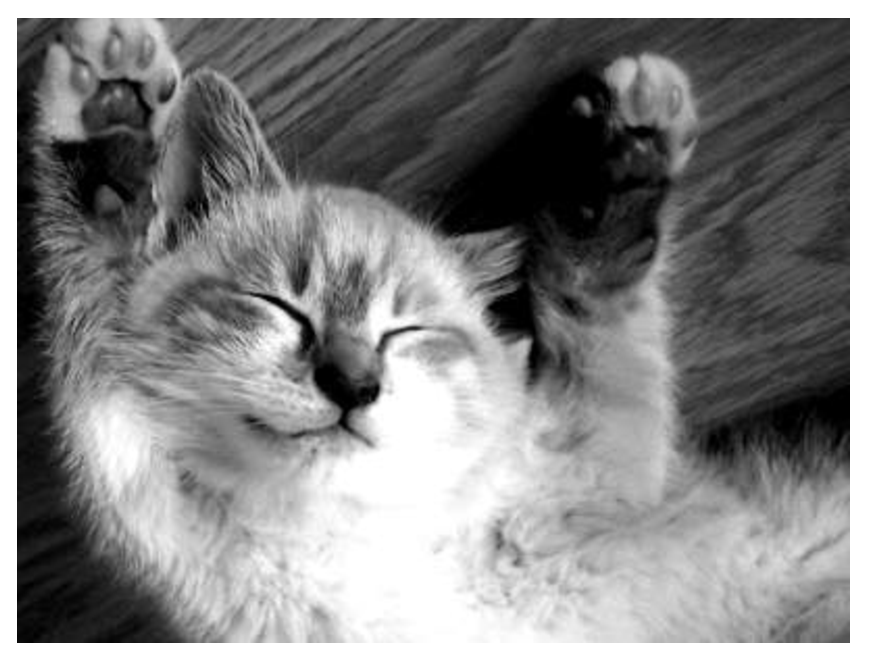
\includegraphics[width=\textwidth]{./chapters/demonstration/no_release/kitten.eps}
  \caption[Case 1DI Buffer Contaminants]{
    The Buffer, component 7 ($F_d=0$), acheives total containment.
    }
  \label{fig:lpIbuff}

\end{minipage}
\hspace{0.05\linewidth}
\begin{minipage}[b]{0.45\linewidth}
  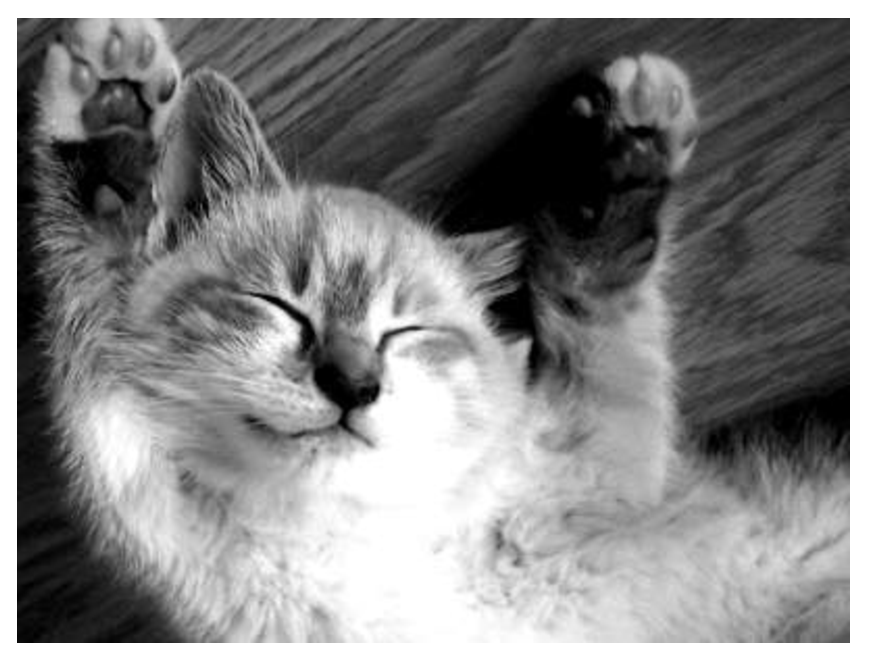
\includegraphics[width=\textwidth]{./chapters/demonstration/no_release/kitten.eps}
  \caption[Case 1DI Waste Package Contaminants.]{ 
    Waste Package 6 ($F_d = 0.1$) recieves then releases material. 
    }
  \label{fig:lpIwp6}

  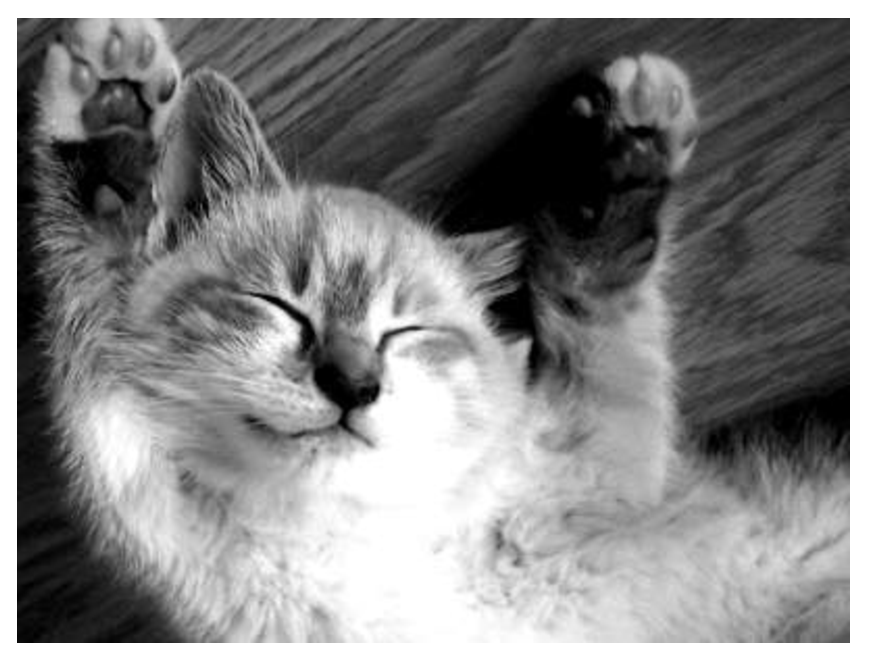
\includegraphics[width=\textwidth]{./chapters/demonstration/no_release/kitten.eps}
  \caption[Case 1DI Waste Package Contaminants.]{ 
    The Far Field, component 0 ($F_d = 0.1$), never recieves material.
    }
  \label{fig:lpIff0}


  \end{minipage}
\end{figure}
\begin{figure}[ht]
\centering
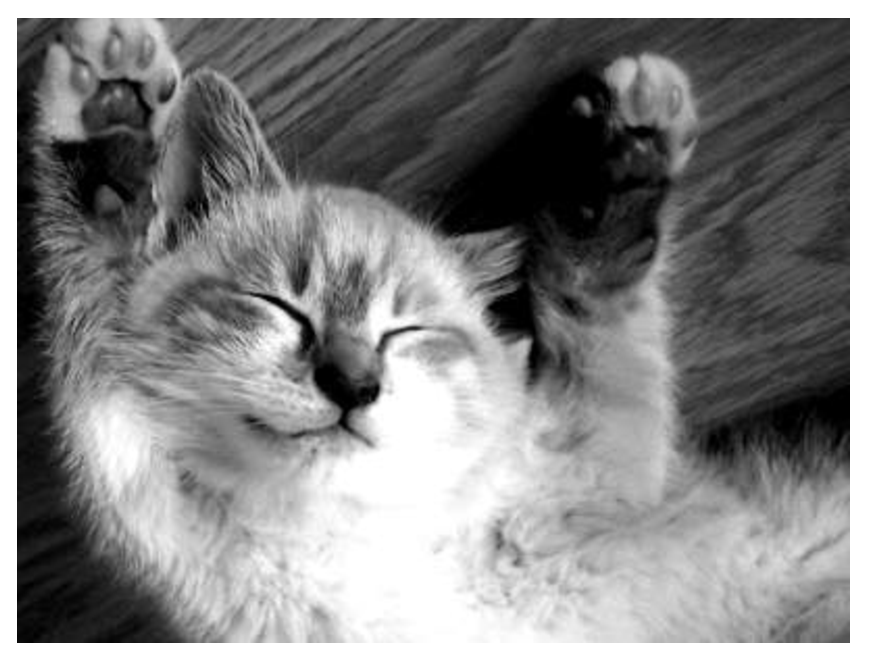
\includegraphics[width=0.8\textwidth]{./chapters/demonstration/no_release/kitten.eps}
\caption[$^{235}U$ residence. Lumped Parameter  <+Component+> No Release.]{
For <+CASE+> case in which total containment in the <+component+> is assumed 
($F_{d,<+comp+>}=0$), $^{235}U$ travels through <++> components ($F_d = 0.1$) before 
permanent residence in the <+component+> component.
}
\label{fig:lpIIall}
\begin{minipage}[b]{0.45\linewidth}

  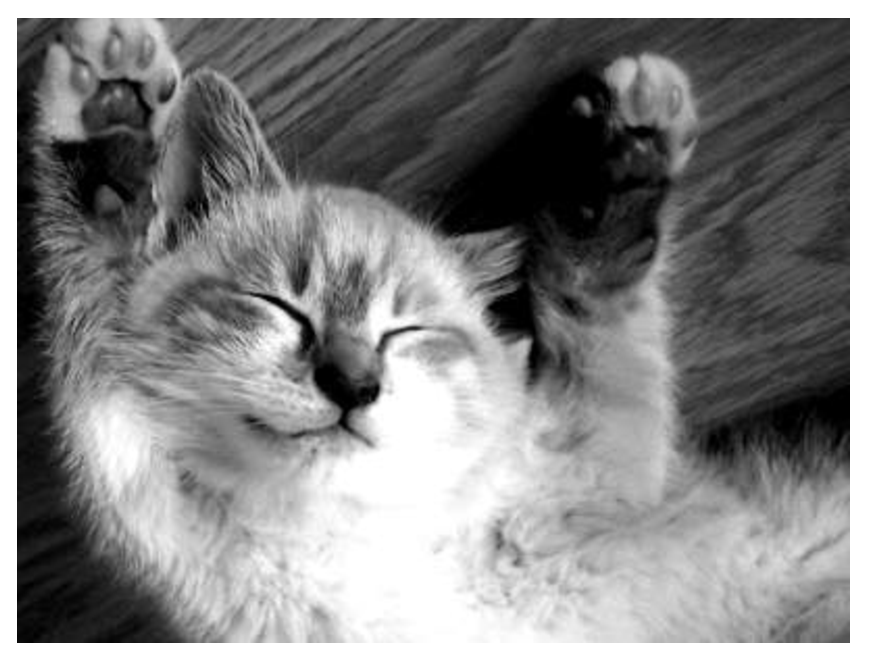
\includegraphics[width=\textwidth]{./chapters/demonstration/no_release/kitten.eps}
  \caption[1DII Waste Form Contaminants.]{
    Waste Form 5 ($F_d = 0.1$) releases material with degradation. 
    }
  \label{fig:lpIIwf5}
  
  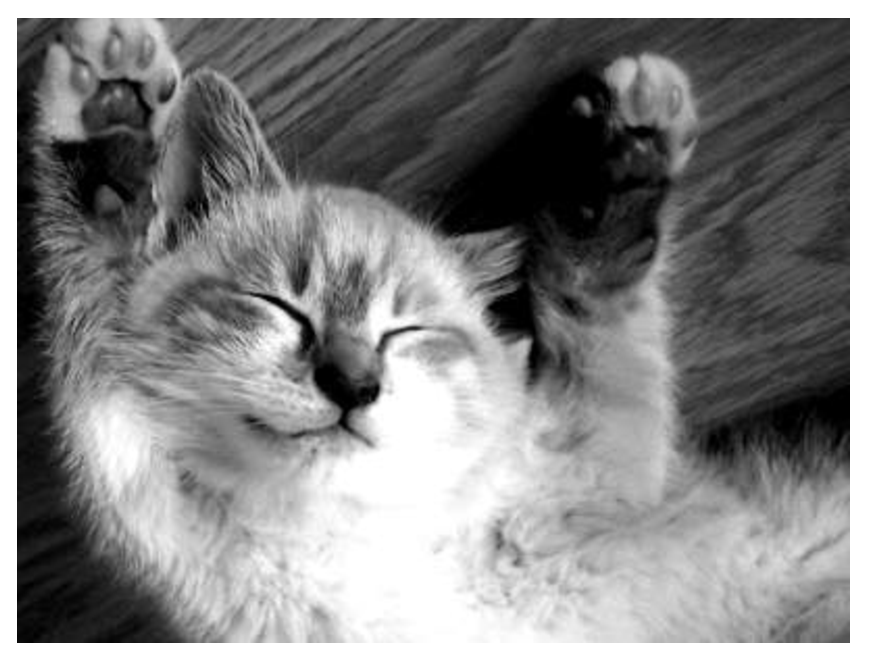
\includegraphics[width=\textwidth]{./chapters/demonstration/no_release/kitten.eps}
  \caption[Case 1DII Buffer Contaminants]{
    The Buffer, component 7 ($F_d=0$), acheives total containment.
    }
  \label{fig:lpIIbuff}

\end{minipage}
\hspace{0.05\linewidth}
\begin{minipage}[b]{0.45\linewidth}
  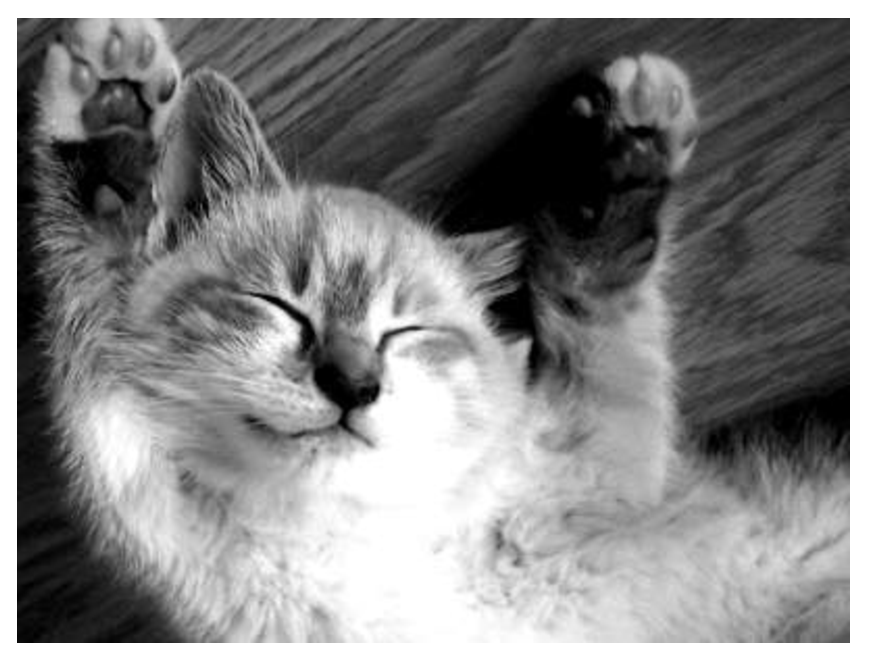
\includegraphics[width=\textwidth]{./chapters/demonstration/no_release/kitten.eps}
  \caption[Case 1DII Waste Package Contaminants.]{ 
    Waste Package 6 ($F_d = 0.1$) recieves then releases material. 
    }
  \label{fig:lpIIwp6}

  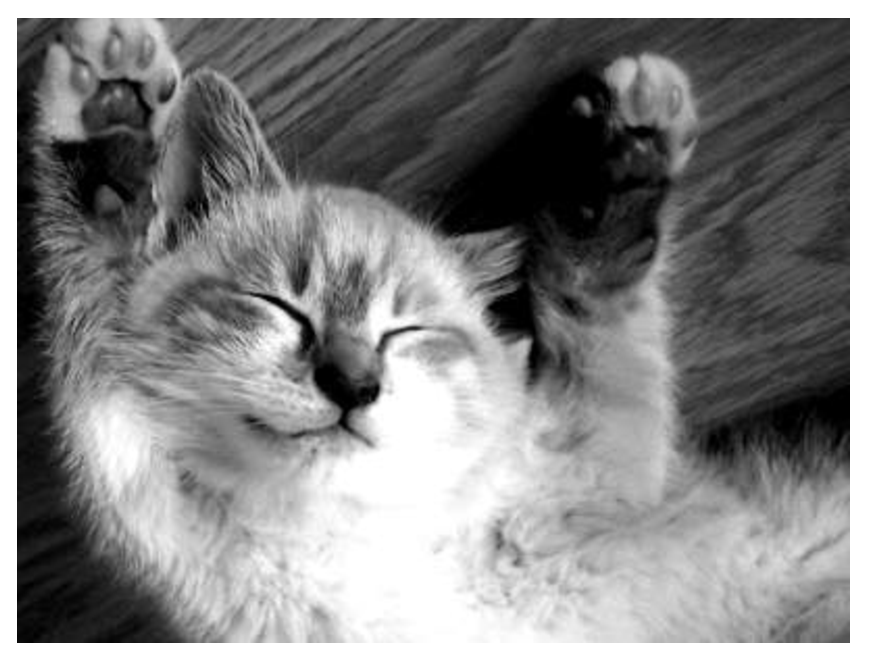
\includegraphics[width=\textwidth]{./chapters/demonstration/no_release/kitten.eps}
  \caption[Case 1DII Waste Package Contaminants.]{ 
    The Far Field, component 0 ($F_d = 0.1$), never recieves material.
    }
  \label{fig:lpIIff0}


  \end{minipage}
\end{figure}
\begin{figure}[ht]
\centering
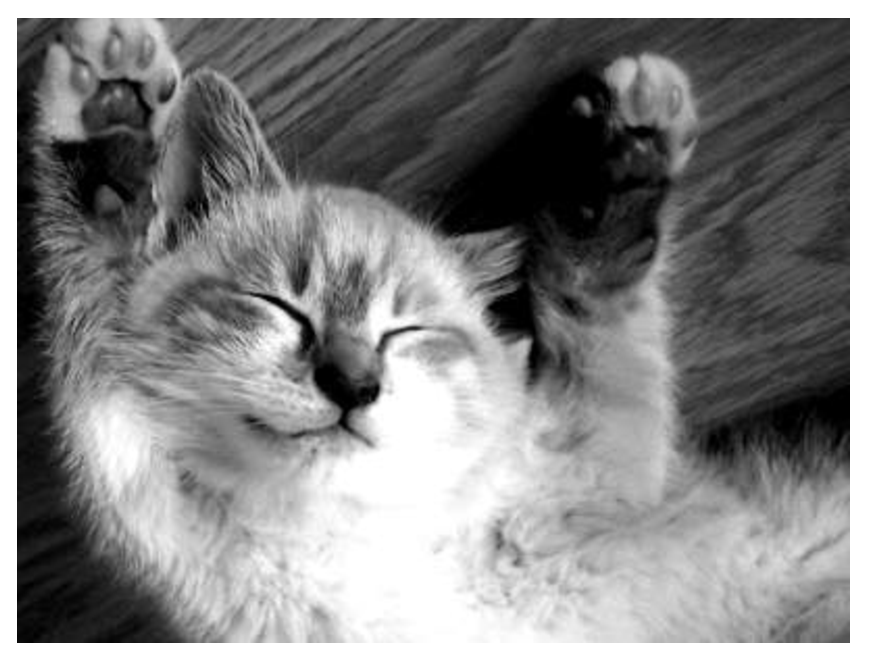
\includegraphics[width=0.8\textwidth]{./chapters/demonstration/no_release/kitten.eps}
\caption[$^{235}U$ residence. Lumped Parameter  <+Component+> No Release.]{
For <+CASE+> case in which total containment in the <+component+> is assumed 
($F_{d,<+comp+>}=0$), $^{235}U$ travels through <++> components ($F_d = 0.1$) before 
permanent residence in the <+component+> component.
}
\label{fig:lpIIIall}
\begin{minipage}[b]{0.45\linewidth}

  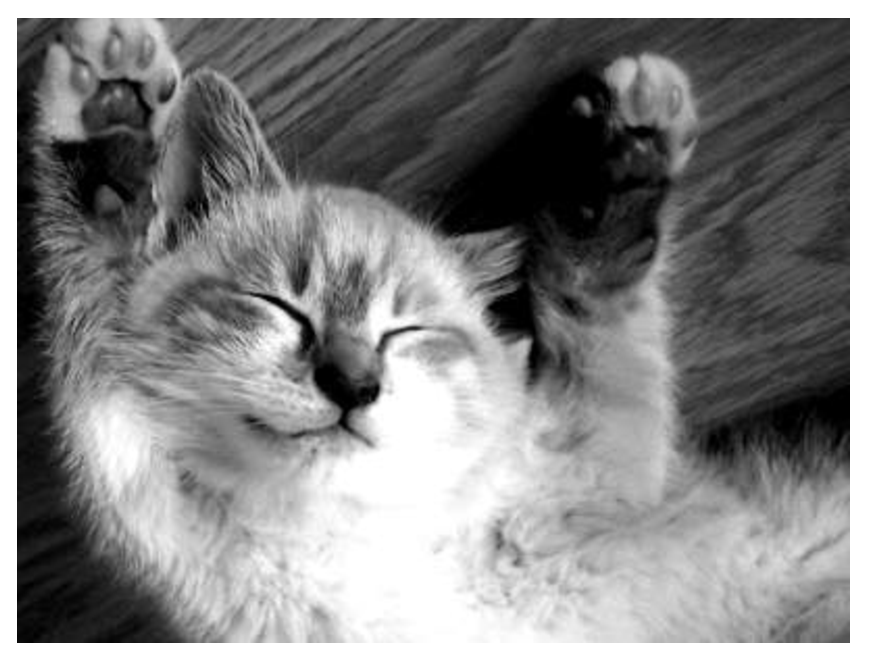
\includegraphics[width=\textwidth]{./chapters/demonstration/no_release/kitten.eps}
  \caption[1DIII Waste Form Contaminants.]{
    Waste Form 5 ($F_d = 0.1$) releases material with degradation. 
    }
  \label{fig:lpIIIwf5}
  
  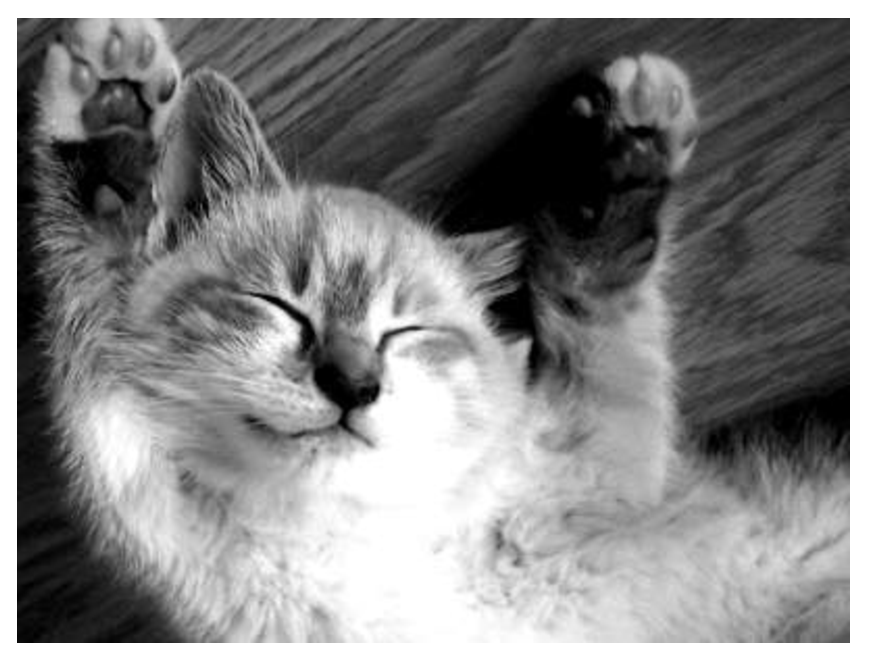
\includegraphics[width=\textwidth]{./chapters/demonstration/no_release/kitten.eps}
  \caption[Case 1DIII Buffer Contaminants]{
    The Buffer, component 7 ($F_d=0$), acheives total containment.
    }
  \label{fig:lpIIIbuff}

\end{minipage}
\hspace{0.05\linewidth}
\begin{minipage}[b]{0.45\linewidth}
  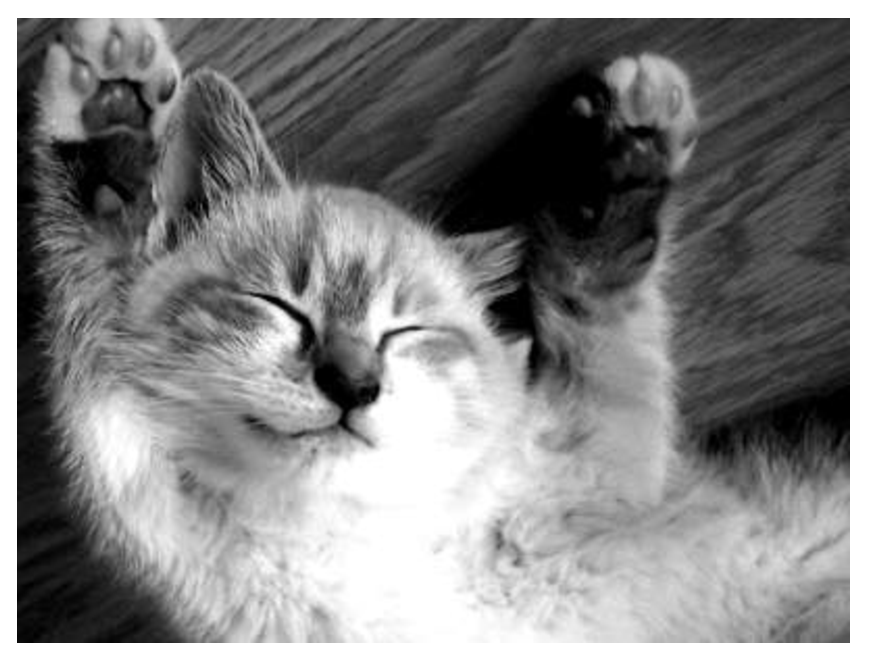
\includegraphics[width=\textwidth]{./chapters/demonstration/no_release/kitten.eps}
  \caption[Case 1DIII Waste Package Contaminants.]{ 
    Waste Package 6 ($F_d = 0.1$) recieves then releases material. 
    }
  \label{fig:lpIIIwp6}

  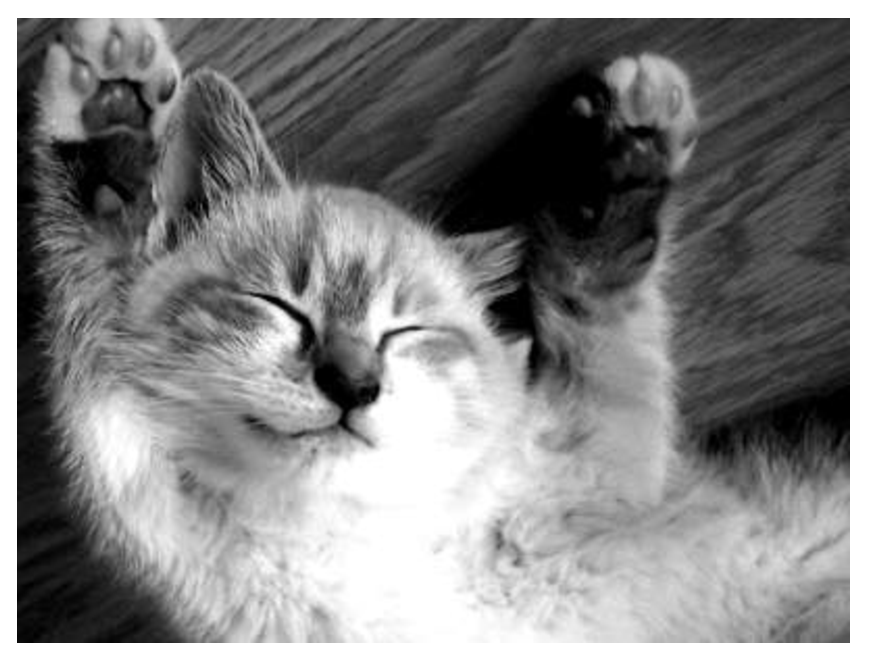
\includegraphics[width=\textwidth]{./chapters/demonstration/no_release/kitten.eps}
  \caption[Case 1DIII Waste Package Contaminants.]{ 
    The Far Field, component 0 ($F_d = 0.1$), never recieves material.
    }
  \label{fig:lpIIIff0}


  \end{minipage}
\end{figure}
\begin{figure}[ht]
\centering
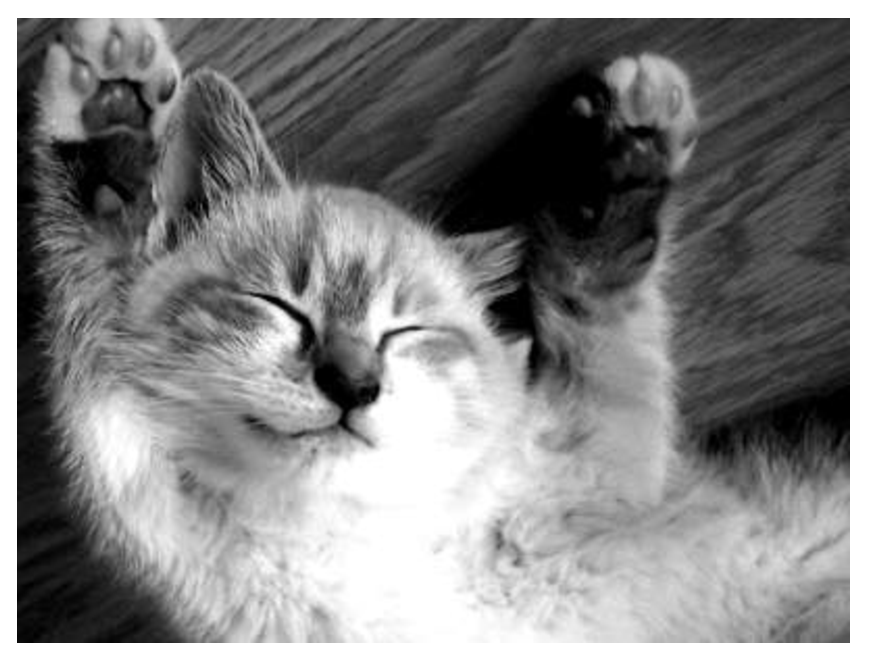
\includegraphics[width=0.8\textwidth]{./chapters/demonstration/no_release/kitten.eps}
\caption[$^{235}U$ residence. Lumped Parameter  <+Component+> No Release.]{
For <+CASE+> case in which total containment in the <+component+> is assumed 
($F_{d,<+comp+>}=0$), $^{235}U$ travels through <++> components ($F_d = 0.1$) before 
permanent residence in the <+component+> component.
}
\label{fig:lpIVall}
\begin{minipage}[b]{0.45\linewidth}

  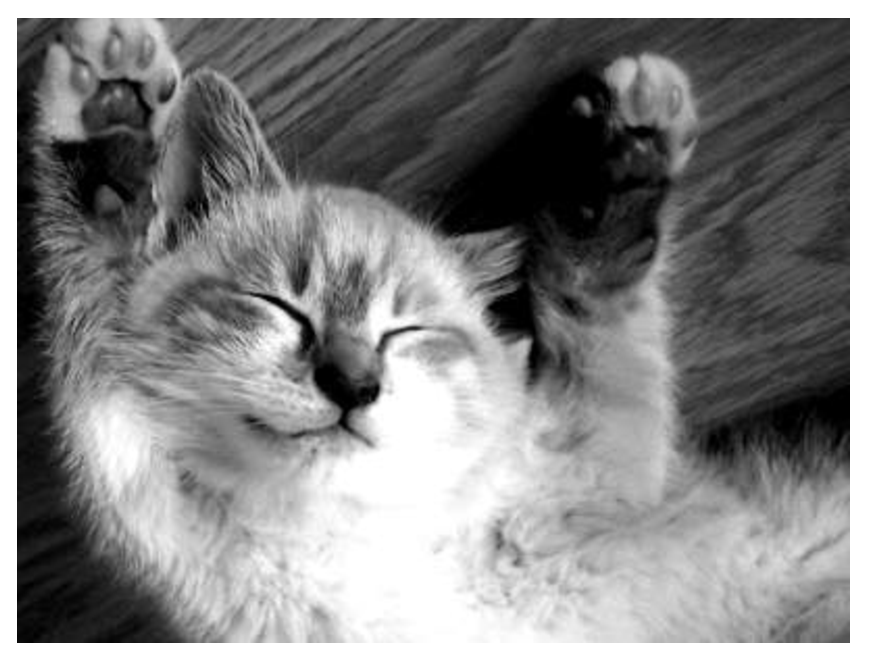
\includegraphics[width=\textwidth]{./chapters/demonstration/no_release/kitten.eps}
  \caption[1DIV Waste Form Contaminants.]{
    Waste Form 5 ($F_d = 0.1$) releases material with degradation. 
    }
  \label{fig:lpIVwf5}
  
  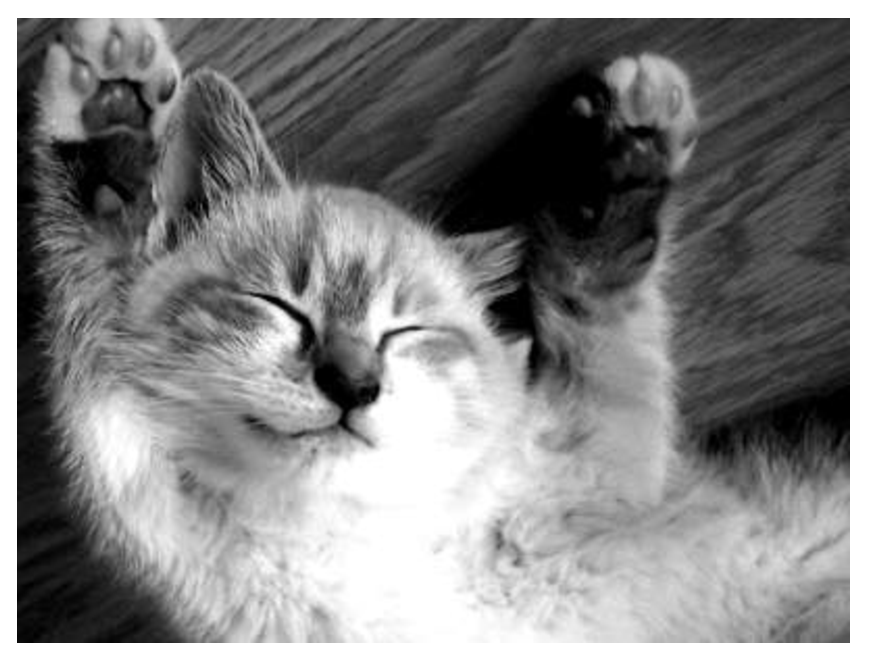
\includegraphics[width=\textwidth]{./chapters/demonstration/no_release/kitten.eps}
  \caption[Case 1DIV Buffer Contaminants]{
    The Buffer, component 7 ($F_d=0$), acheives total containment.
    }
  \label{fig:lpIVbuff}

\end{minipage}
\hspace{0.05\linewidth}
\begin{minipage}[b]{0.45\linewidth}
  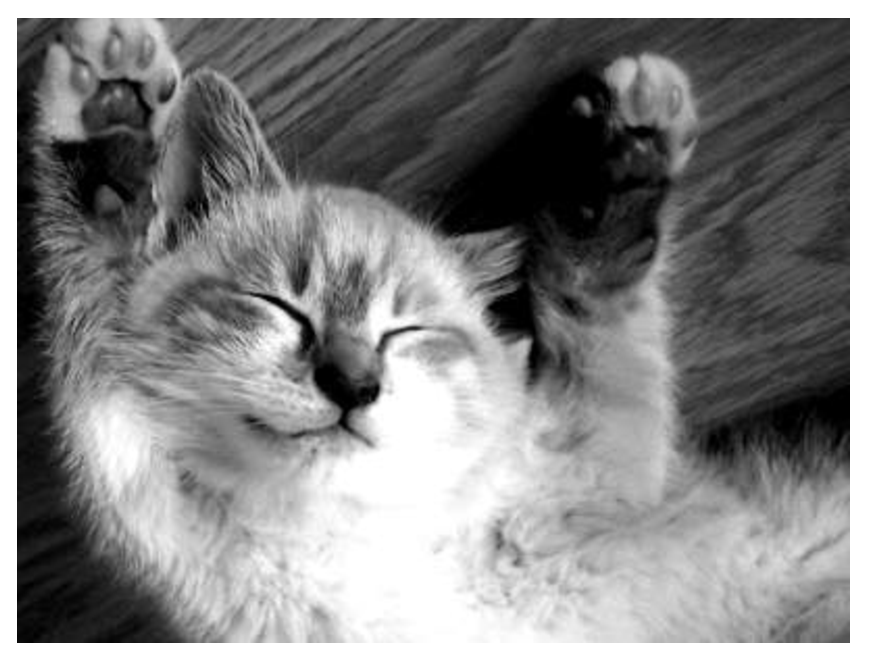
\includegraphics[width=\textwidth]{./chapters/demonstration/no_release/kitten.eps}
  \caption[Case 1DIV Waste Package Contaminants.]{ 
    Waste Package 6 ($F_d = 0.1$) recieves then releases material. 
    }
  \label{fig:lpIVwp6}

  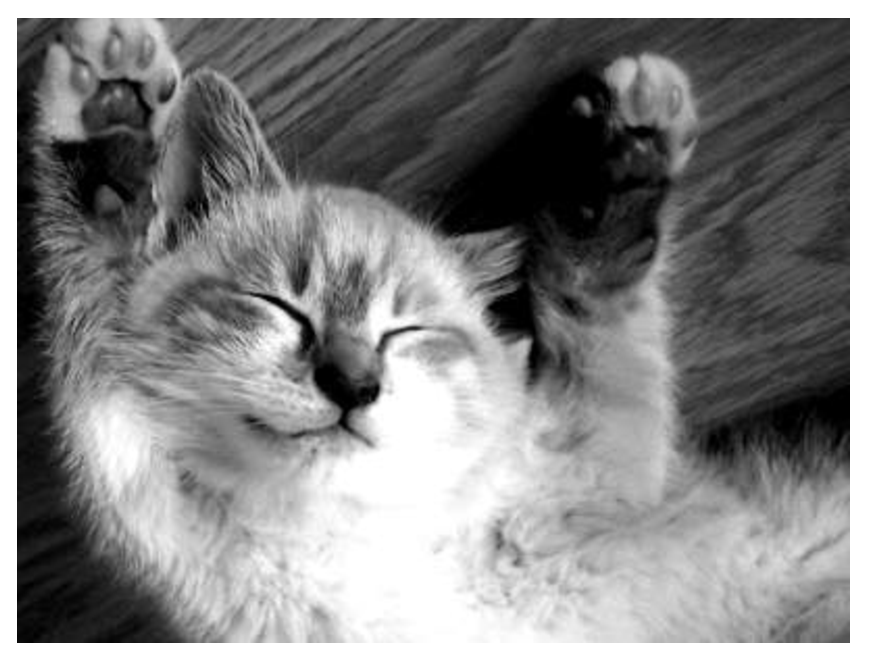
\includegraphics[width=\textwidth]{./chapters/demonstration/no_release/kitten.eps}
  \caption[Case 1DIV Waste Package Contaminants.]{ 
    The Far Field, component 0 ($F_d = 0.1$), never recieves material.
    }
  \label{fig:lpIVff0}


  \end{minipage}
\end{figure}
